%\documentclass[9pt]{pnas-new}
%\templatetype{pnasresearcharticle} % Choose template
\documentclass[9pt]{article}
\usepackage[english]{babel}

\usepackage{amsmath}
\usepackage{graphicx}
\usepackage[colorlinks=true, allcolors=blue]{hyperref}

\title{Collective Behaviour Report 1 : Simulating Schooling Fish Feeding Behaviour}
\author{Melinda Fabien, Sarah Gay, Ana Gelez and Alina Sereda}
%\affil{Collective behaviour course research seminar report}
%\leadauthor{Fabien}

%\significancestatement{Simulating Schooling Fish Feeding Behaviour}{In this article we present a simulation of a school of fish in a tank. We were interested in modeling the behavior of fishes in order to find the optimal way to feed them. We explain our simulation model and discuss our implementation. Then we discuss the results and how we can improve our simulation to take more data into account and provide more realistic results.}{}


%\dates{\textbf{\today}}
%\program{BM-RI}
%\vol{2023/24}
%\no{CB:GI} % group ID

\begin{document}
\maketitle

\begin{abstract}
In this article we present a simulation of a school of fish in a tank. We were interested in modeling the behavior of fishes in order to find the optimal way to feed them. We explain our simulation model and discuss our implementation. Then we discuss the results and how we can improve our simulation to take more data into account and provide more realistic results.
\end{abstract}

\section{Introduction}


Estimating optimal living conditions for fish in aquaculture can be challenging due to the expense, time, and potential harm to the fish involved in traditional testing methods. In the referenced paper \cite{article}, the authors proposed various testing methods for optimizing the distribution system in a simulated fish tank environment. The aim is to optimize the feeding distribution system in aquaculture, thereby improving management and creating conditions for accelerated fish growth, all while saving time and resources. 

Although this simulation provides significant results that can be used, it is also limited since it only applies to the rainbow trout species.  Furthermore, it neglects considerations of other environmental variables, such as the possibility of fish mortality resulting from malnutrition. 

The goal of our project is to enhance this highly promising simulation by incorporating additional features.The initial step is to reproduce this simulation using our own means. After obtaining the first results, we will discuss to identify relevant and feasible extensions. If we find them beneficial, they will be integrated into our model.


\section{Method}

Our main work for this first step has been to reproduce the original simulation. To achieve this goal, we had to understand precisely how it works and then implement it with Godot Engine.

\subsection{Proposed simulation Model}

The simulation provided by the article is divided into two main parts: Feeding and Growth. These two phases alternate simultaneously until reaching a certain limit (either a specified number of days or a predefined time) or reaching a capacity limit in the aquarium.

\subsubsection{Feeding simulation}

In this section, we focus on the way the fish are fed. In the initial iterations, we chose default values of 38.53cm. This value was derived from studies conducted in the following study \cite{morales1994effects}, specifically for rainbow trout. However, it is fish-specific and would need adaptation if we intend to extend this experiment to other fish species.

The model individually evaluates the amount of food ingested by each fish, taking into account the fish's size and mass. 
Whenever a fish comes into contact with a pellet, the cumulative count of pellets it has encountered increases. Then, we used this count to calculate the `feed\_intake\_weight`, which involves multiplying the weight of a pellet with the number of pellets ingested by the fish during this phase. Currently, we are only considering the size of the pellet in our model.

\subsubsection{Growth simulation}

Following the Feeding Simulation phase, we enter the Growth phase. Depending on the quantity of food ingested by the fish in the previous phase, it will experience varying degrees of growth. To accurately calculate this, we employ the Feed Conversion Efficiency (FCE).

The choice of FCE being set to 1.0 is deliberate. A value of 1.0 for FCE implies that all the ingested food contributes directly to the fish's body mass gain. This simplification is used to maintain straightforward relationship between feed intake and growth, especially since we don't have more information about their metabolic system. 

After the body mass was updated, total length was calculated from the following allometric equation:

\[W_n^i = (a \times TL_n^i)^b\] 

where \(TL_n^i\) is the total length of the i-th individual on the n-th day and a and b are coefficients of allometry; here, a was 0.0209 and b was 2.843, respectively

It is equally important to prevent excessive daily growth in fish size. To address this, we implement a safeguard by establishing a maximum size the fish can achieve in a single day, capped at 4\% of the fish's body mass.

\subsubsection{Movement model of the fish}

Each fish adheres to the following movement model:

\[W_n^i a_{t+\Delta t} = F_t\]
\[v_{t+\Delta t} = v_t +  a_{t+\Delta t}*\Delta t\]
\[x_{t+\Delta t} = x_t + v_{t+\Delta t} *\Delta t\]


Depending on whether there is food in the aquaculture tank or not, the fish's movement model will change.

\begin{figure}[h]
    \centering
    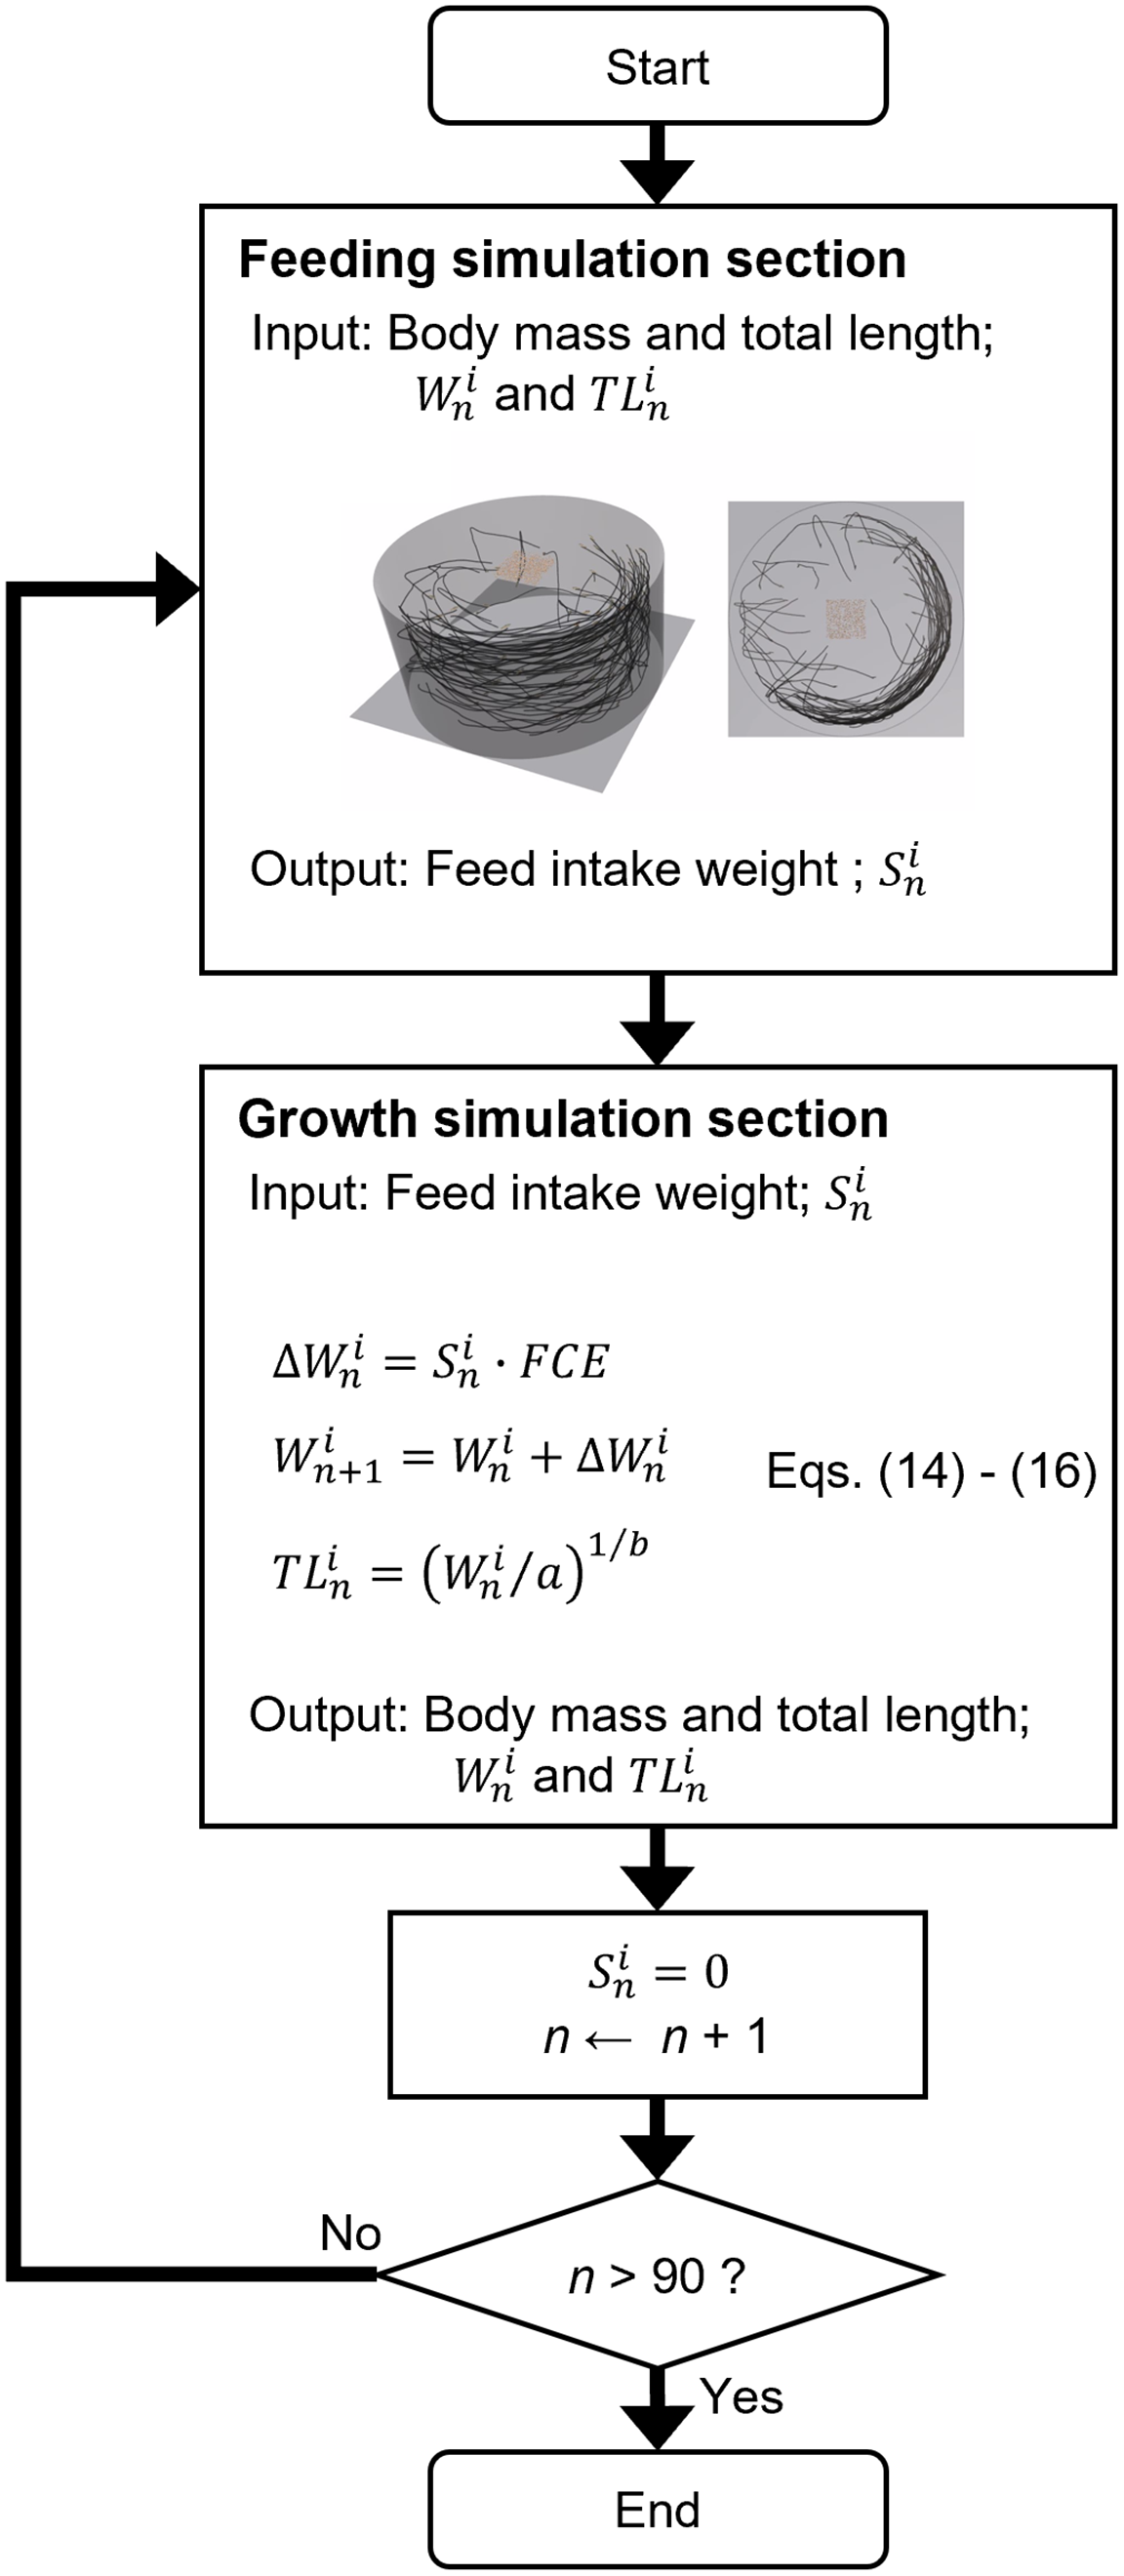
\includegraphics[width=0.3\linewidth]{figure3.PNG}
    \caption{Simulation Model}
    \label{fig:figure1}
\end{figure}

During the feeding phase (see Figure \ref{fig:figure1}), the fish will move more quickly towards the food. The vector v5 \(TL_n^i\) corresponding to vector in our model, transitions from 0 to 3 if the fish is not satiated (i.e., it has not exceeded the maximum size it can gain in a day). The speed coefficients used in the movement equations are also adjusted to change from 1.5 to 7.


We have also implemented movements related to "fish schooling ," among the following six: 


\begin{itemize}
    \item \textbf{Separation} :  Moves away from the nearest individual.
    \item \textbf{Alignment} : Moves in the same direction as others.
    \item \textbf{Cohesion }: Vector directed towards the center of other individuals within the field of view
    \item  \textbf{Approaching feed} :  Attracts force towards food.
    \item \textbf{avoiding boundary} : Repulsive force from boundary 
    \item Random movement : Move randomly 
\end{itemize}

To see the details of the equation, refer to this article \cite{article}

\subsection{Setup and visualization of the fish}
We decided to both simulate and visualize the fish behaviour with Godot Engine which is a tool quite similar to Unity. It uses its particular programming language, GDScript, which is Python inspired. For the simulation, we used two classes : Food and Fish. The tank and its details is created in the main so the bulk of the function is in the two first classes.
\begin{itemize}
    \item \textbf{Food} : This one is the simplest and set the weight and the movement of the pellet once dropped into the tank
    \item \textbf{Fish} :  This class takes care of simulating the size and behaviour of fish but also the two phases explained above. It manages the modification in behaviour when food is detected by fish, the growth when eating food and the collective behaviour of the school as mentioned.
\end{itemize}   




\section{Results}

Currently, we have successfully implemented the food distribution system. To generate a food item, a simple click on the screen is sufficient, triggering the appearance of the food. Additionally, we have established the tank environment where the fish can swim and have implemented the underlying logic of the swimming force.

\begin{figure}[h]
    \centering
    \begin{minipage}[b]{0.45\linewidth}
        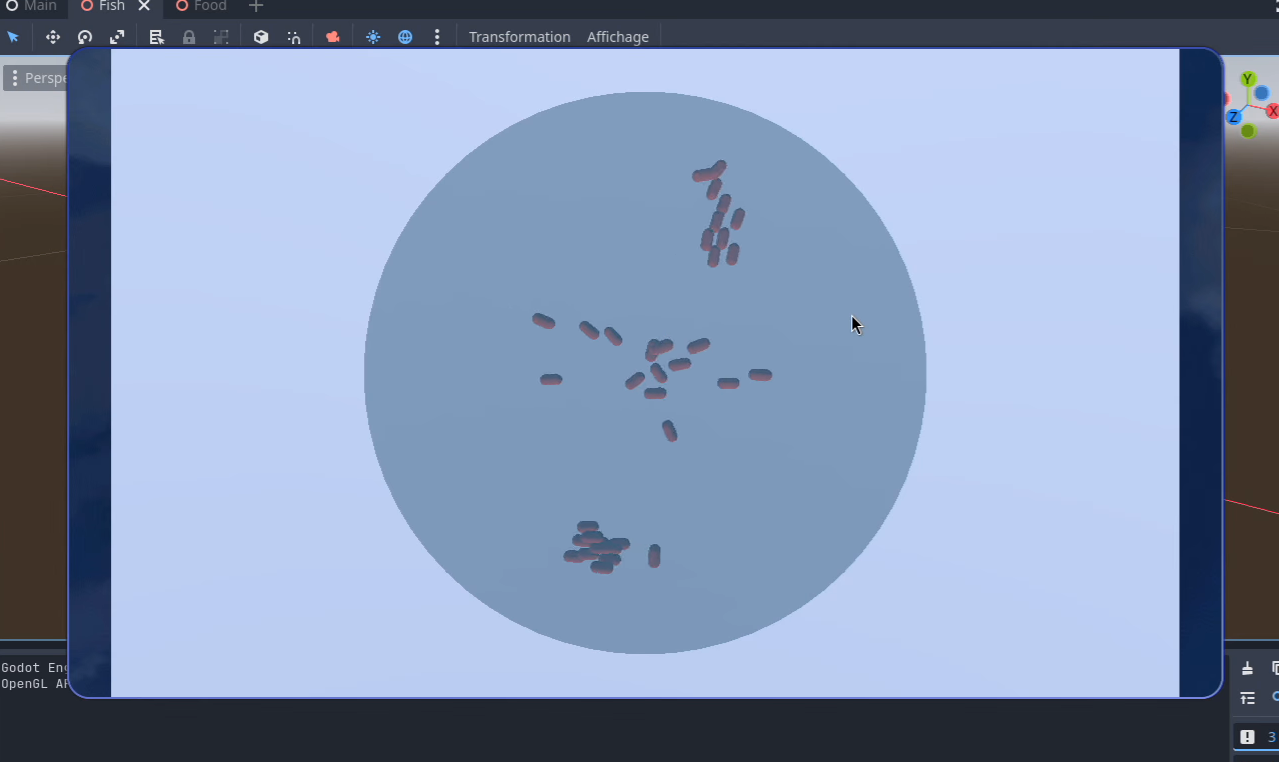
\includegraphics[width=\textwidth]{Capture.PNG}
        \caption{Top View of the simulation}
        \label{fig:Top view tankl}
    \end{minipage}
    \hspace{0.5cm}
    \begin{minipage}[b]{0.45\linewidth}
        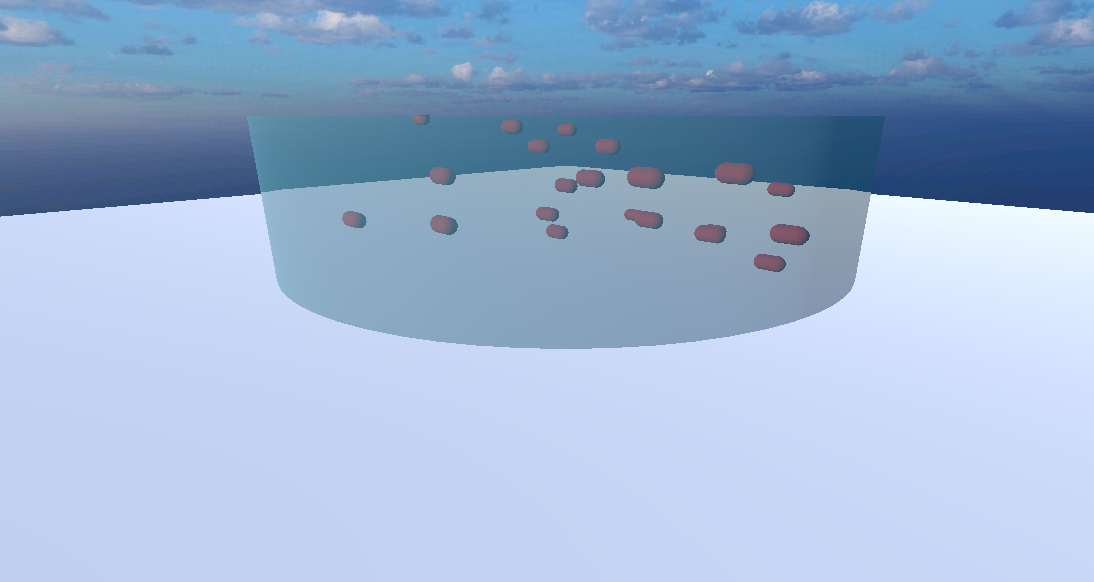
\includegraphics[width=\textwidth]{poisson2.png}
        \caption{View of the simulation}
        \label{fig: basic view tankl}
    \end{minipage}
\end{figure}

We've implemented behavioural aspects into the fish schooling movement, including food attraction. When there's food in the tank, the fish move faster. Additionally, certain fish can form groups and behave like it, while also avoiding boundaries.



\section{Discussion}
\subsection{What are the future tasks ?}
For now we have almost implemented the simulation presented in the paper. The only thing that needs to be done in this regard is the dropping area of the pellet. Indeed, the main observation of the paper rests on the pellet distribution area. As we can see on the figure size, the food can be distributed in a centered square of 0.5m, 1m or 1.5m but in our simulation, we drop only one pellet at a time so we have to implement a feeding area with multiple pellets. 

\begin{figure}
    \centering
    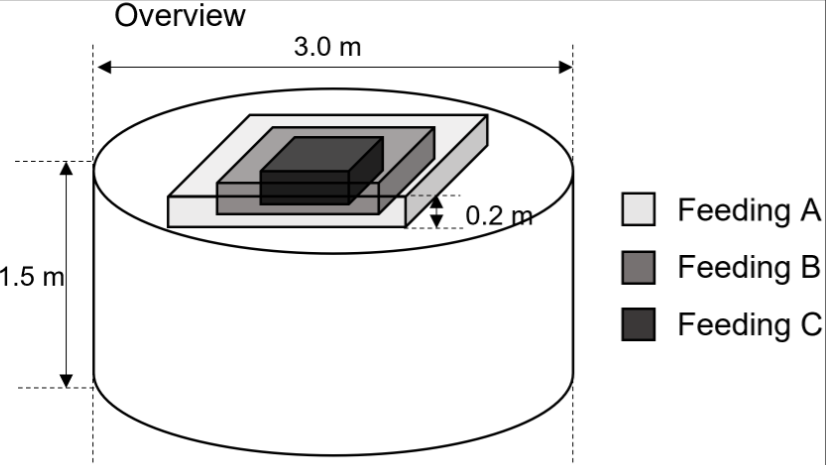
\includegraphics[width=0.3\linewidth]{fig5.png}
    \caption{Simulation field}
    \label{fig:enter-label}
\end{figure}

After this step we will add further details such as integrate a pellet counter to track fish food consumption. Additionally, we will automate the food distribution system for simplified management. We will introduce a limiting feature, either in terms of time or the number of fish, for precise control over simulation parameters. Visual improvements are also in progress to make the environment more appealing.

Once this has been done, we will have reached the stage of the original simulation and will compare our results to the ones provided. With these we will be able to add the most relevant extensions in our context.


\subsection{What kind of extensions can be added?}
We already have several ideas about which extensions to add that can be sorted by category. Each extensions wont require the same amount of modifications and we have to consider the feasibility of each of them. Here's what we've already thought of :

\small\subsubsection*{Feeding parameters}
\begin{itemize}
    \item Different feeding areas : line shape, cross shape, multiple points around the tank, etc.
    \item Increasing or reducing pellet weight.
\end{itemize}

\small\subsubsection*{Fish life}
\begin{itemize}
    \item Reproduction according to age and environment
    \item Use the DEB model instead of the Feed Conversion Efficiency to have more realistic metabolism.
    \item Death by malnutrition after a certain time.
    \item Other type of fish : we found a paper providing a lot of information about Atlantic salmon \cite{handeland2008effect} that can be used to see how a different species acts under the same conditions.
\end{itemize}

\small\subsubsection*{Particularity of aquaculture}
\begin{itemize}
    \item Oxygen management that could lead to death by asphyxiation.
    \item Remove fish when they reach a certain weight.
\end{itemize}


\section{Conclusion }
To summarize what has been done, we now have nearly reproduced the model proposed in the original paper with the exception of food distribution area. We have also planned the next steps which are to automate the food dropping and the population of fish management and to discuss the extensions that will be implemented in order to make the simulation more realistic.


\bibliographystyle{alpha}
\bibliography{sample}
\end{document}
